
\subsubsection*{Problem definition}

The aim of this example is to simulate the transport of a tracer by molecular diffusion in an anisotropic porous medium. The side length of the square numerical model is 1~m. At the left corner at the bottom of the model a constant concentration is diffusing into the calculation area. Diffusion is the only process for tracer transport, there are no pressure differences in the whole area. Because of the anisotropy of the soil material the tracer has to diffuse much faster in x-direction than in vertical direction. This has to be evaluated by comparing the concentration distributions in both directions.

\subsubsection*{Model set-up of the 2~D numerical model}

As initial condition the pressure and tracer concentration were set to 0 in the whole area. At the left corner at the bottom of the model a concentration relation c/c$_0$ of 1 is specified along two polylines of the length of 0.3~m. The boundary conditions correspond to the initial conditions. The calculation model includes 736 triangular elements and 409 nodes. Table \ref{tab55} shows the used parameters for the simulation. As the porous medium is assumed to be anisotropic, which influences diffusion, the value for tortuosity is set equal to 1 in x-direction and 0.1 in y-direction.

\begin{table}[htbp]
\centering
\begin{tabular}{|l|l|l|}
\hline
parameter & value & unit \\
\hline
porosity $\Phi$ & 0.4 & -- \\
\hline
permeability $K$ & 1.0$\cdot 10^{-15}$ & m$^2$ \\
\hline
density water $\rho$  & 1000 & kg/m$^{-3}$  \\		
\hline	
viscosity water $\eta$ & 0.001 & Pa$\cdot$ s \\
\hline	
dispersion length & 10.0 & m \\
\hline
diffusion coefficient D$_a$ & 6.0$\cdot 10^{-10}$ & m$^2$/s  \\
\hline
\end{tabular}
\caption{Used parameters}
\label{tab55}
\end{table}

The calculation is made for 30 time steps with a length of 1$\cdot$10$^7$ seconds. The calculation model is sketched in figure \ref{fig511}.

\begin{figure}[htbp]
\centering
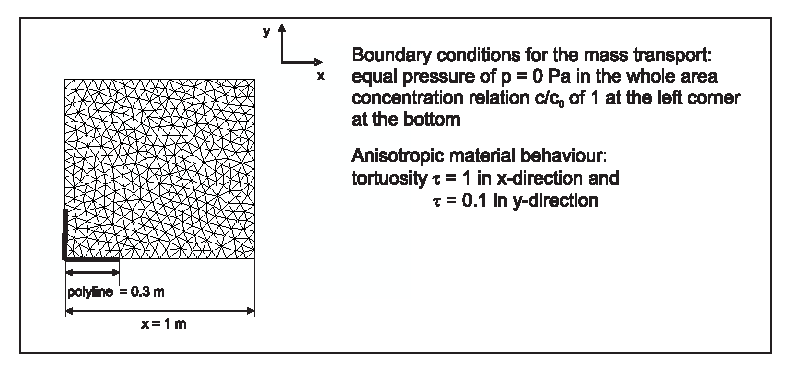
\includegraphics[width=0.9\textwidth]{C/figures/fig511.eps}
\caption{Calculation model (2D)}
\label{fig511}
\end{figure}

\subsubsection*{Evaluation method}
As the process of diffusion is dependent on the actual concentration in the porous medium and on the point in time, an analytical solution for the present calculation model is not possible. Therefore, the results of the RockFlow simulation are solely evaluated in a qualitative way by comparing the concentration distributions in horizontal and vertical direction.

\begin{figure}[htbp]
\centering
\includegraphics[width=0.8\textwidth]{C/figures/fig512.EPS}
\caption{Concentration distributions in x- and y-direction}
\label{fig512}
\end{figure}

\subsubsection*{Results}

In figure \ref{fig512} you can find the concentration distributions over the model side length of 1~m in x- and y-direction, respectively, after a simulation time of 1$\cdot$10$^8$ seconds. Assuming a small tortuosity of 0.1, the component is not yet transported over the whole transport length of 1~m in vertical direction, while in horizontal direction the concentration relation equals approximately 0.3 at the opposite border of the model. The shown trend in the change of diffusion velocity by assuming different tortuosities in x- and y-direction in order to specify anisotropic material behaviour for molecular diffusion has a comprehensible characteristic.

\begin{tabular}{|l|l|l|}
\hline
Benchmark & Problem type	& Path in benchmark deposit \\
\hline	
diff\_aniso	& HC	& benchmarks $\backslash$HC$\backslash$Diffusion$\backslash$ \\
\hline	
\end{tabular}
